%
% File writeup.tex
%
%% Based on the style files for ACL-2015, with some improvements
%%  taken from the NAACL-2016 style
%% Based on the style files for ACL-2014, which were, in turn,
%% based on ACL-2013, ACL-2012, ACL-2011, ACL-2010, ACL-IJCNLP-2009,
%% EACL-2009, IJCNLP-2008...
%% Based on the style files for EACL 2006 by 
%%e.agirre@ehu.es or Sergi.Balari@uab.es
%% and that of ACL 08 by Joakim Nivre and Noah Smith

\documentclass[11pt,a4paper]{article}
\usepackage[hyperref]{writeup}
\usepackage{graphicx}
\usepackage{times}
\usepackage{latexsym}

\usepackage{url}

\aclfinalcopy % Uncomment this line for the final submission

\newcommand\BibTeX{B{\sc ib}\TeX}

\title{ %
  Congestion-Control Algorithms on an Emulated Cellular Network\\
\large CS 244 PA2 Writeup}

\author{Hope Casey-Allen  \\
  {\tt hcaseyal@stanford.edu} \\\And
  Jiaxin Guan \\
  {\tt jxguan@stanford.edu} \\}

\date{}

\begin{document}
\maketitle
\begin{abstract}
  This document contains the instructions for preparing a camera-ready
  manuscript for the proceedings of ACL-2017. The document itself
  conforms to its own specifications, and is therefore an example of
  what your manuscript should look like. These instructions should be
  used for both papers submitted for review and for final versions of
  accepted papers.  Authors are asked to conform to all the directions
  reported in this document.
\end{abstract}



\section{Fixed Window Size}
\label{sec:fixed}

\subsection{Varying the Window Sizes}
We created a script to vary the fixed window size and output results for average
capacity, average throughput, 95th percentile per-packet queueing delay, and
95th percentile signal delay (see \texttt{datagrump/warmup-a.sh}). We took measurements
with windows sizes of $1$, $2$, $5$, $10$, $20$, $50$, $100$, $200$, $500$ and
took them over $3$ runs
each to estimate the repeatability of the measurements. The results we had are
shown in figure \ref{fig:warmup-a}.
\begin{figure}[h]
  \centering
  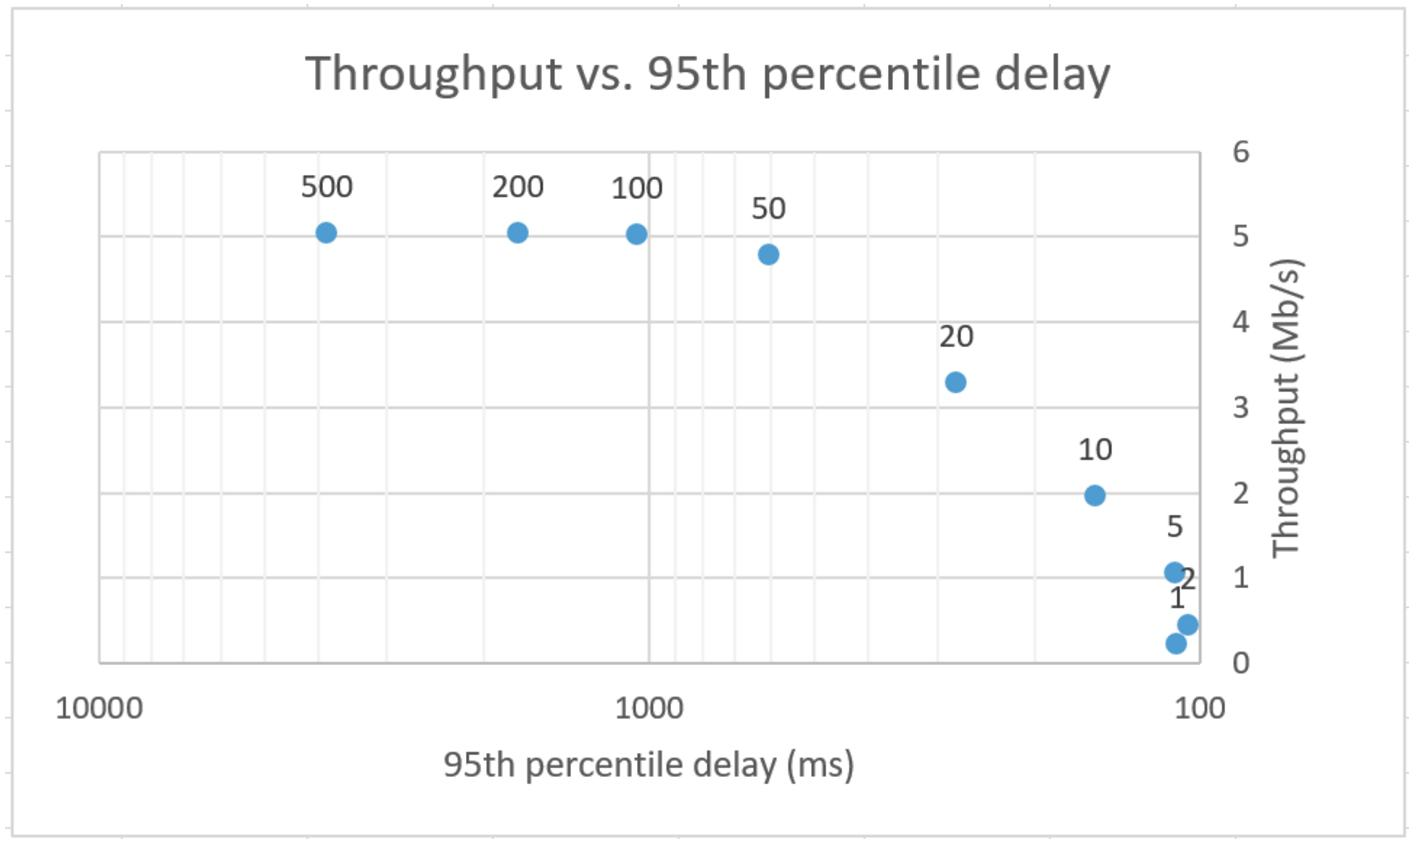
\includegraphics[scale=0.15]{warmup-a}
  \caption{The performance for different fixed window sizes. Data Labels
  represent the corresponding fixed window size.}
  \label{fig:warmup-a}
\end{figure}

We can observe an overall pattern that by increasing the window size, we're able
to obtain better network utilization, but at the same time getting higher delay.
This matches our expectation as we would expect the queue to be full and the
network fully utilized for large fixed window sizes.

Another interesting observation is that when increasing the window size
from $1$ to $2$, the throughput increases, while at the same time the delay also
slightly decreases. This is interesting in that normally we would expect the
delay to increase as we increase the window size. We suspect that it is because
with a
larger window size $2$, which is still way smaller than the network capacity, more
packets can be sent through the network when the network is not at all
congested. In this way, we have more packets with low delay for window size $2$,
and hence a lower average delay.

Notice that this reasoning only applies
to window sizes that are way smaller than the max network capacity, because with
relatively large window sizes, the network is likely often fully utilized -
increasing the window size would not lead to more packets being delivered with
low delay, but rather it will lead to more packets waiting in the queue when the
network is congested, and hence a higher average delay.

\subsection{Best Fixed Window Size}
By examining the
results from section $1.1$, we observed that the window size that maximized the
overall score was between $5$
and $20$. 
We then reran the script, but this time varying the input window size
parameter between $5$ and 
$20$ to perform a ternary search to find the exact best window
size. The resulting best fixed window size that we found is $12$, with a score of
$12.84$ using the $\texttt{throughput}/\texttt{delay}$ function on the contest page (or
$3.68$ if using the $\log(\texttt{throughput}/\texttt{delay})$  function on the assignment
handout).
This is not a great result, but it is more than $10$ times better than
the performance for fixed window size $1$.

\subsection{Repeatability}

We calculated the standard deviation for our results for the best fixed window
size over $10$ runs (see table \ref{tab:warmup-a}). We can see that the standard
deviations are very low when compared to the averages, showing that the
measurements are extremely repeatable. This matches our expectation because
all of the code is deterministic. The only source of variations is likely the
fluctuation of the machine performance or different shceduling decisions.

\begin{table}[h]
  \centering
  \begin{tabular}{|c|r|r|}
    \hline
                         & \multicolumn{1}{c|}{StdDev} &
    \multicolumn{1}{c|}{Avg} \\ \hline
    Throughput (Mbits/s) & 0.005                       & 2.263
    \\ \hline
    Delay (ms)           & 0.333                       & 175.889
    \\ \hline
    Score                & 0.046                       & 12.868
    \\ \hline
  \end{tabular}
  \caption{The standard deviations and averages of the throughput, delay and
  overall score.}
  \label{tab:warmup-a}
\end{table}


\section{Additive Increase, Multiplicative Decrease (AIMD)}
\label{sec:aimd}

\subsection{Implementation}

We implemented the AIMD scheme in \verb|datagrump/controller.cc|. We made a slight modification that we perform
a multiplicative decrease whenever the RTT exceeds a specific timeout. This
simulates the situations where packets get lost in transmission and are resent
after a timeout (conventionally $2* \texttt{RTT}$). We derived the actual RTT by using
the timestamps in the \texttt{ack\_received} function per the Piazza post. We
tested the implementation first with arbitrarily set constants, which gave us a score
around $18$, which is a significant improvement over the fixed window size
algorithm.

\subsection{Choosing the Constants}

In order to choose the constants that yield the best performance, we first wrote a
script to try different constants of additive increase
size and multiplicative decrease factor. We were able to get the result shown
in table \ref{tab:warmup-b}.

\begin{table}[h]
  \centering
  \begin{tabular}{|c|r|r|r|r|r|}
    \hline
    \multicolumn{1}{|l|}{} & \multicolumn{1}{c|}{1} & \multicolumn{1}{c|}{2} &
    \multicolumn{1}{c|}{4} & \multicolumn{1}{c|}{8} & \multicolumn{1}{c|}{16} \\
    \hline
    0.2                    & 18.52                  & 18.55                  &
    14.97                  & 12.91                  & 10.65                   \\
    \hline
    0.4                    & 18.71                  & 18.75                  &
    14.74                  & 12.79                  & 11.06                   \\
    \hline
    0.6                    & 17.37                  & 18.67                  &
    14.95                  & 12.98                  & 10.63                   \\
    \hline
    0.8                    & 17.99                  & 18.33                  &
    15.30                  & 13.24                  & 10.76                   \\
    \hline
  \end{tabular}
  \caption{The scores for different additive increase sizes and multiplicative
  decrease factors. The rows are the different factors for the multiplicative
decrease, and the columns are the factors for the additive increase.}
  \label{tab:warmup-b}
\end{table}
  
  We can observe from the table that the optimal performance occurs with an
  additive increase size of $2$ and a multiplicative decrease factor of $0.4$.
  So we fixed these two constant and varied on the initial window size, which
  yielded the following result in figure \ref{tab:warmup-b2}.

  \begin{figure}[h]
  \centering
  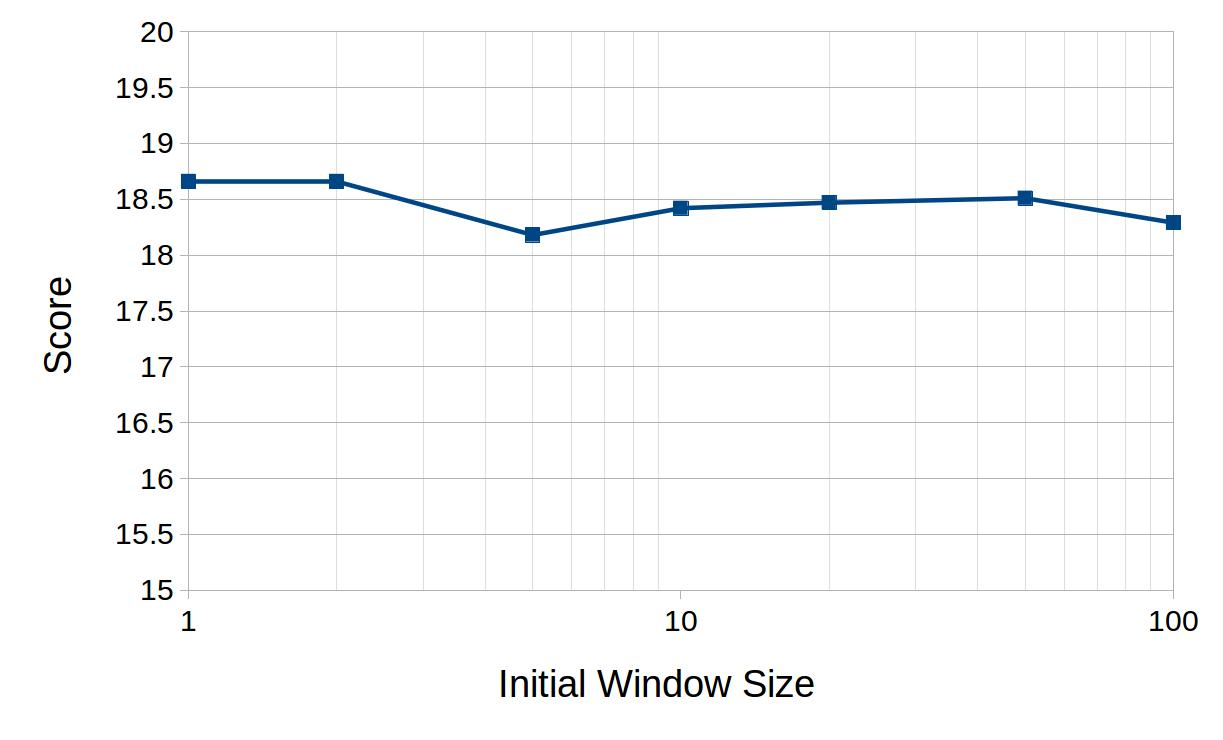
\includegraphics[scale=0.35]{warmup-b}
  \caption{The distribution of scores over different initial window sizes.}
  \label{tab:warmup-b2}
\end{figure}

  We can see from the figure that the score is not influence much by the initial
  window size. It merely fluctuates around $18.5$. This meets our expection, as
  the initial window size only matters for the very first few clock cycles.
  Hence, we picked the initial window size to be $2$, which yielded the highest
  score in our testing.

  Notice that we did not tune the timeout constant, mainly for two reasons:
  \begin{enumerate}
    \item In an AIMD scheme, the timeout is conventionally simply $2 *
      \texttt{RTT}$.
      With the average RTT estimation of $105$ ms from section \ref{sec:fixed},
      we set the timeout to be $210$ ms.
    \item Notice that since our timeout is based on the timestamp when the ACK
      is received by the sender and the timestamp when the sender sends the
      packet, it essentially the delay used in delay-triggered schemes.
      Therefore, we will tune the threshold later in section \ref{sec:delay}.
  \end{enumerate}

  Bringing these parts together, the final constants that we choose for the AIMD
  scheme are:
  \pagebreak
  \begin{verbatim}
  INITIAL_WINDOW_SIZE = 2
  ADDITIVE_INCREASE_SIZE = 2
  MULT_DECREASE_FACTOR = 0.4
  MD_TIMEOUT = 210
  \end{verbatim}

  These constant yielded a score of $18.66$, which is around $1.5$ times the
  fixed window size algorithm.

\subsection{Analysis}

Overall, the AIMD scheme that we implemented did quite good in utilizing the
network with a network utilization of almost $90\%$. However, it's not doing so
well in signal delay, the average of which is well above $200$ ms. Since the
score is calculated as $\texttt{throughput}/\texttt{delay}$, with such a high delay, even if we
could achive $99.9\%$ utilization, the score would still be capped at around
$25$. We would
definitely need some other, not necessarily more sophisticated, algorithm to
achieve high throughput and low delay.

\section{Delay-Triggered Schemes}
\label{sec:delay}
Since in the AIMD implementation we used received ack timestamps to determine if
a timeout
occurred, the AIMD scheme we have implemented in section \ref{sec:aimd} is
essentially a delay-trigger scheme by itself. While we've tuned the AIMD
constants in section \ref{sec:aimd}, in this section, we will be tuning the
RTT threshold for the delay, as well as exploring other options to update the window
size. 

\subsection{Tuning the Threshold}

Again, we set up a script to test the score under differnt thresholds. The
results are shown in figure \ref{fig:warmup-c}.

\begin{figure}[]
  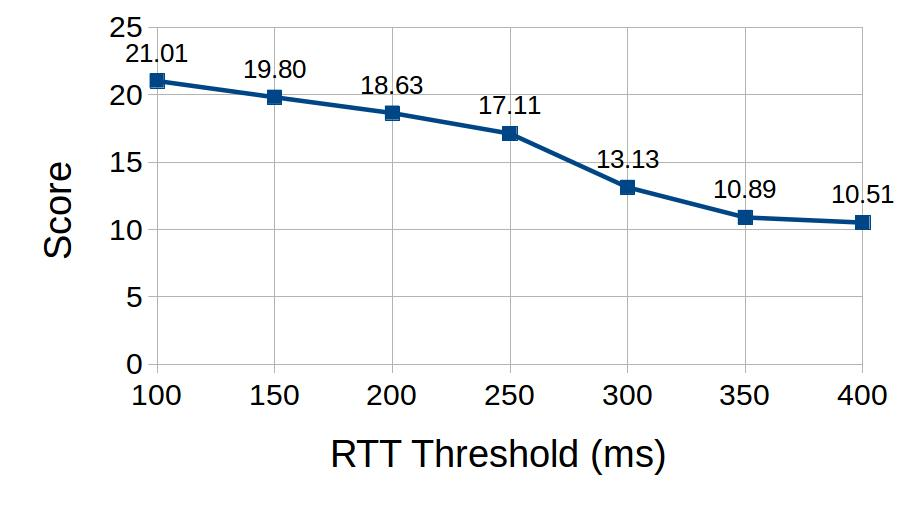
\includegraphics[scale=0.45]{warmup-c}
  \caption{The score distribution over different RTT thresholds.}
  \label{fig:warmup-c}
\end{figure}

We can see an overall trend of decreasing score as the RTT threshold increases.
Therefore, we also explicitly tested the case where the RTT threshold is $50$ ms. Since the
lowest possible RTT (propagation delay) is around $42$ ms, the threshold of $50$
ms yielded
very bad utilization, as the AIMD scheme is constantly switching between the
additive increase phase and the multiplicative decrease phase. It was easy to
tell that the $50$ ms threshold has a dissatisfying score (we did not even bother
to wait for
it to finish as we can already tell from the ongoing graph).

Therefore, in the end, we chose the RTT threshold to be $100$ ms, which gave us
the best result with a score of $21.01$.

\subsection{Additive Increase, Additive Decrease (AIAD)}
\label{ssec:aiad}
We also experimented with different ways to update window size based on the
delay.

One thing that we tried is an AIAD scheme with both the increase size and
the decrease size being $2$. We can see from the result in figure \ref{fig:aiad}
that there is a very high utilization of $96.6\%$. But by using a
additive decrease rather than multiplicative decrease, this algorithm's reaction to
high delays is really slow, leading to an average signal delay of $361$ ms. The
overall score given by this algorithm is only $13.49$, merely surpassing the
fixed window size algorithm.

\begin{figure*}[h]
  \centering
  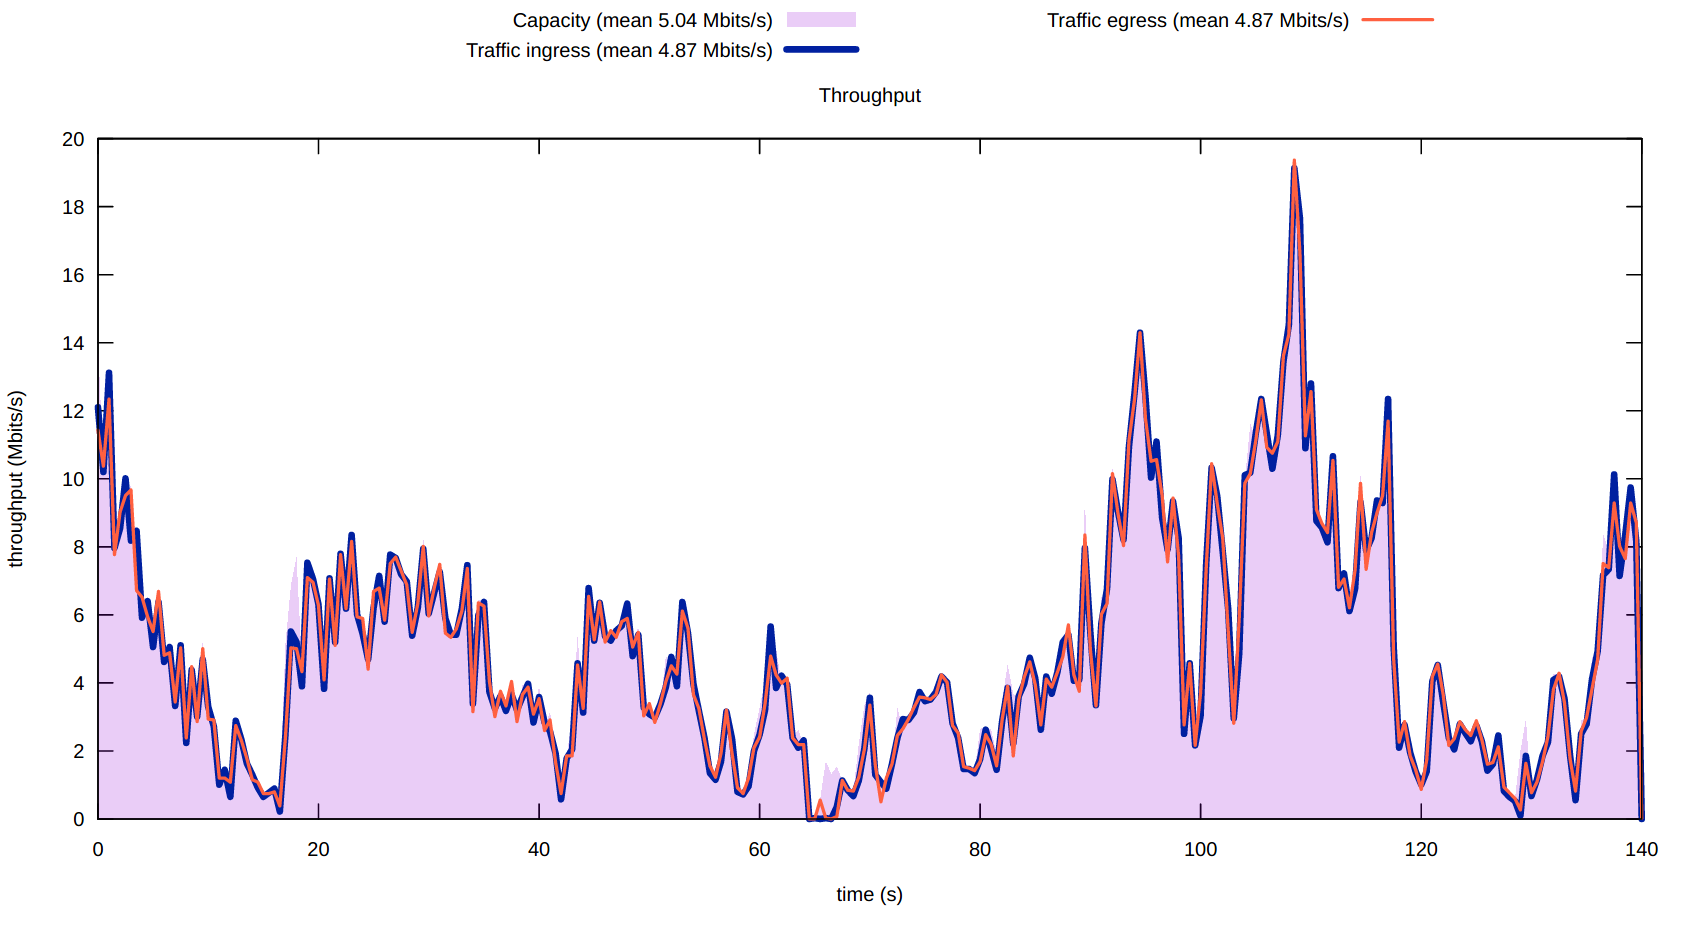
\includegraphics[scale=0.2]{aiad}
  \caption{The result of an AIAD scheme with both additive increase size and
  additive decrease size equal to $2$.}
  \label{fig:aiad}
\end{figure*}
\subsection{Multiplicative Increase, Multiplicative Decrease (MIMD)}

As a complement to section \ref{ssec:aiad}, we also experimented with an MIMD
scheme with the multiplicative increase factor set to be $1.1$ and the
multiplicative decrease factor set to be $0.5$. From figure \ref{fig:mimd}, we
can see that, as we have expected, the multiplicative increase is too aggressive,
sending way too many packet than what the network can handle, leading to a very
high signal delay. Also from figure \ref{fig:mimd2}, we can clearly see that all
the high delays are caused by the spikes of sent packets during the
multiplicative increase phase. However, the utilization seems quite good with a $90.6\%$
utilization rate, because there are always
tons of packets waiting to be delivered in the queue. But since the delays are
so high, the overall score for this
MIMD scheme is only $0.1$, by far the third to last on the "leaderboard".

\begin{figure*}[h]
  \centering
  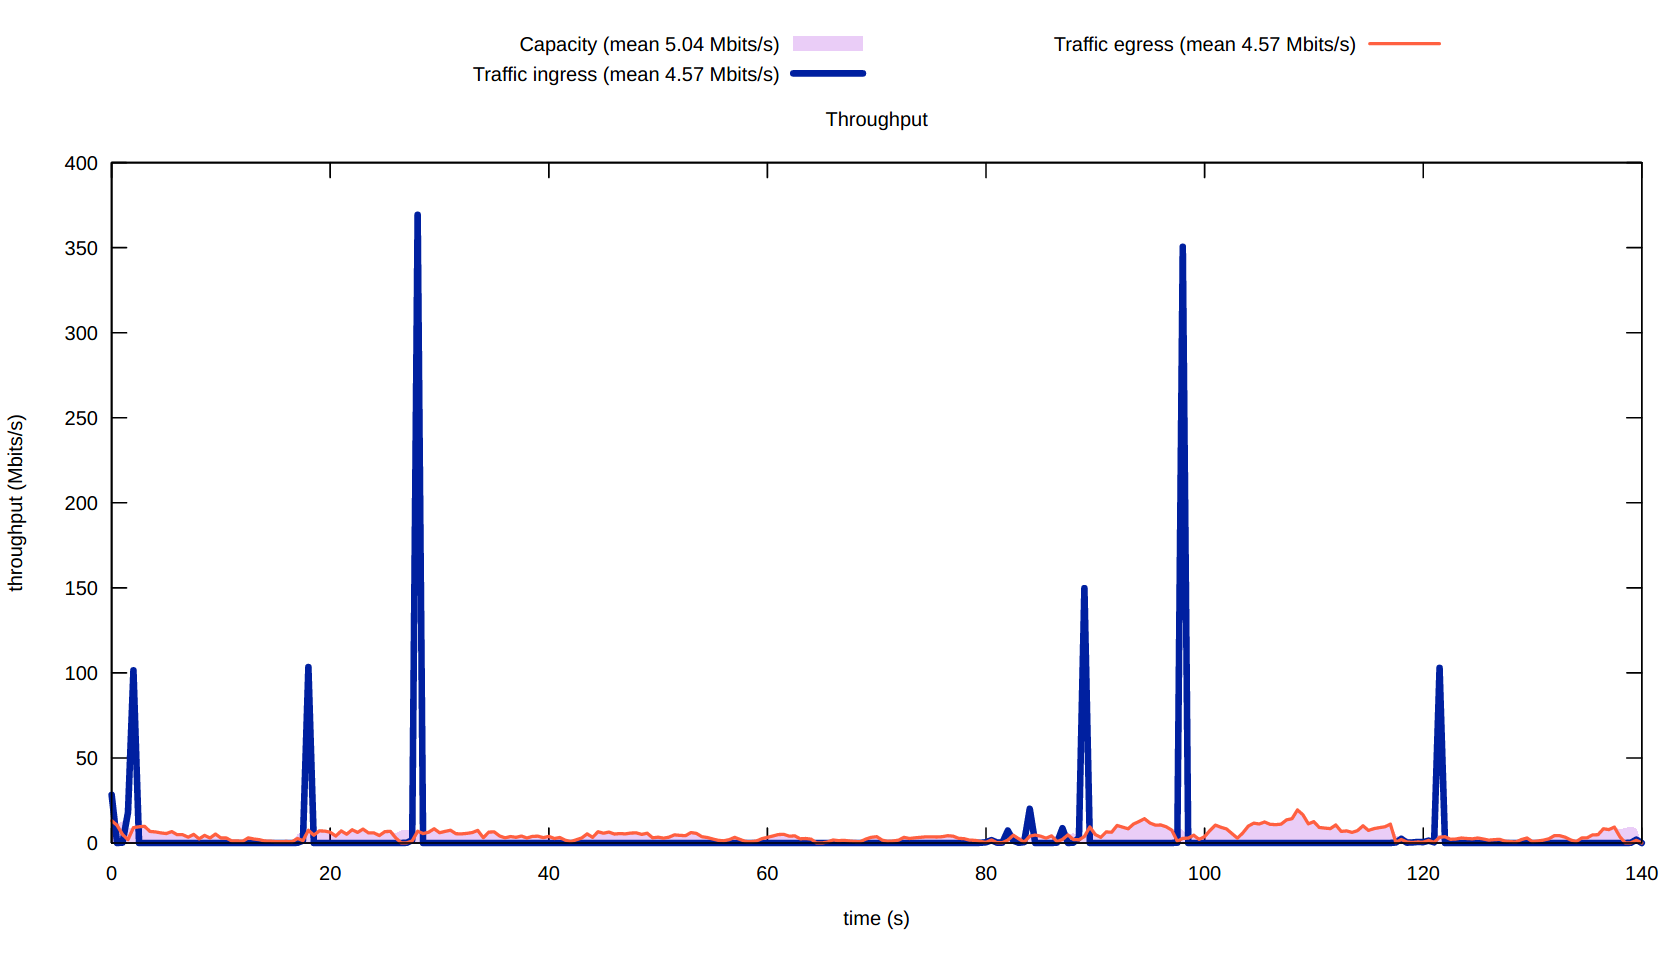
\includegraphics[scale=0.2]{mimd}
  \caption{The result of an MIMD scheme with multiplicative increase factor
    $1.1$ and multiplicative decrease factor $0.5$.}
  \label{fig:mimd}
\end{figure*}

\begin{figure*}[h]
  \centering
  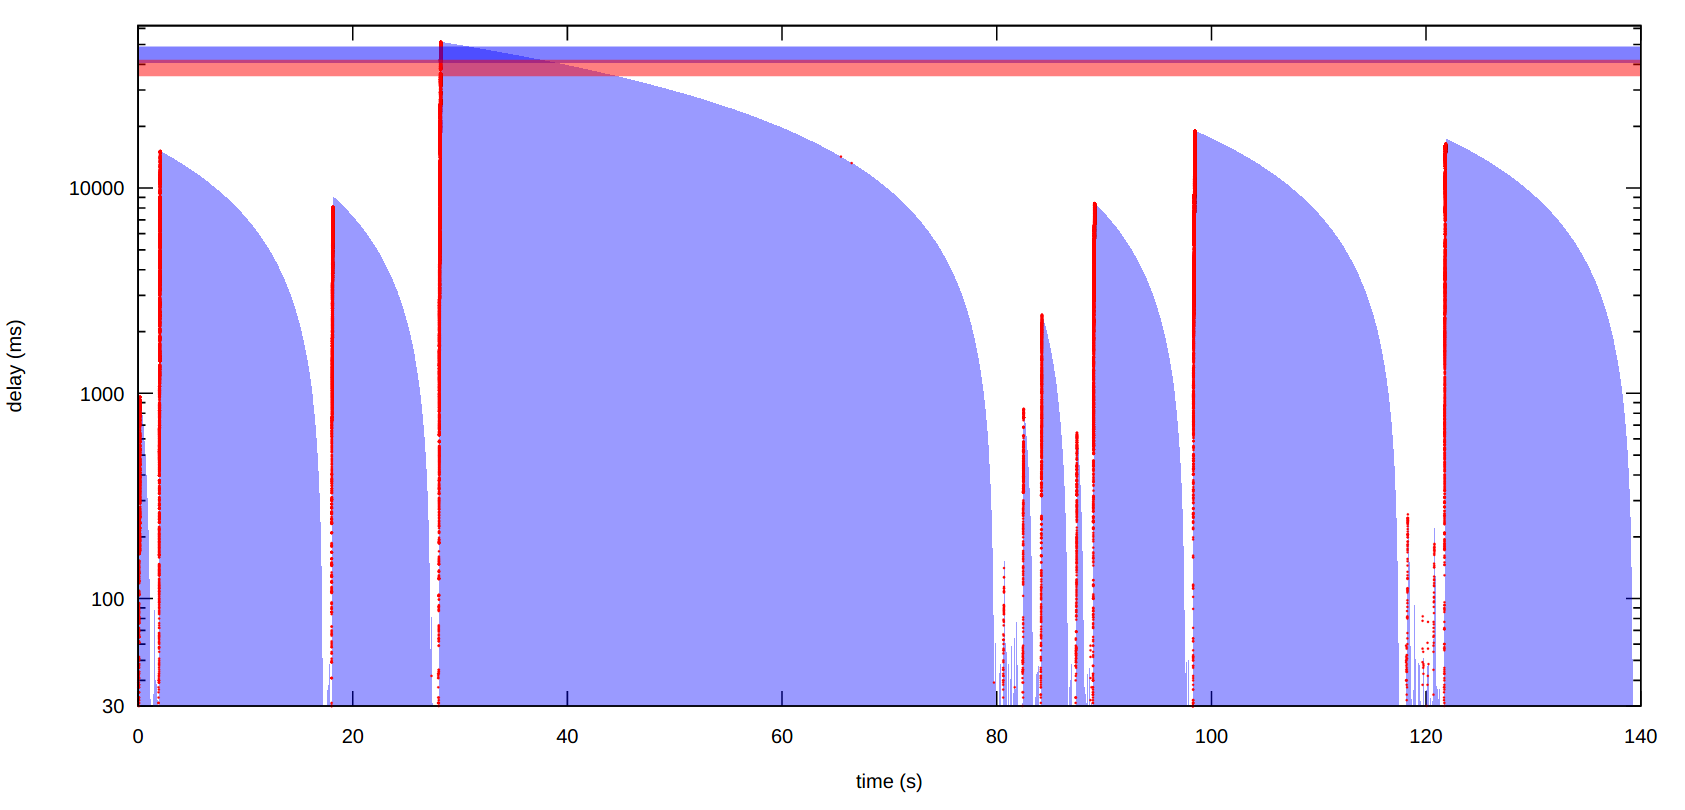
\includegraphics[scale=0.2]{mimd-2}
  \caption{The delay over time for the MIMD scheme with multiplicative increase factor
    $1.1$ and multiplicative decrease factor $0.5$.}
  \label{fig:mimd2}
\end{figure*}

\subsection{Lesson Learned}

Neither the AIAD and the MIMD scheme seems ideal, so in order to achieve a
better performance, we would probably want to start from the AIMD scheme and see
what optimizations we can add to it.

\section{The Contest}
\subsection{Starting Out: Researching Related Work}

We started our approach by watching the Sprout video and skimming the Sprout
source code and the Sprout paper \cite{winstein2013stochastic}. We really liked the idea that Sprout presented of predicting network
capacity changes in order to achieve high throughput and low delay. 

We also read \textit{Timely: Rtt-based Congestion Control for the Datacenter}
\cite{mittal2015timely} and liked
the idea of using delay gradients to adjust transmission rate. We also
appreciated how it is simlar to the AIMD scheme by endorsing the
additive increase and multiplicative decrease phases. However, we were
aware that we may not be able to make RTT measurements with microsecond accuracy
and thus the delay gradients may not be totally sufficient to estimate switch
queueing. 

\subsection{Delay Gradient Scheme}
The first scheme we tried was based off of the delay gradient scheme presented
in the \textit{Timely} paper \cite{mittal2015timely}.  We took advantage of the
following pseudocode from the paper:

\begin{algorithm}
  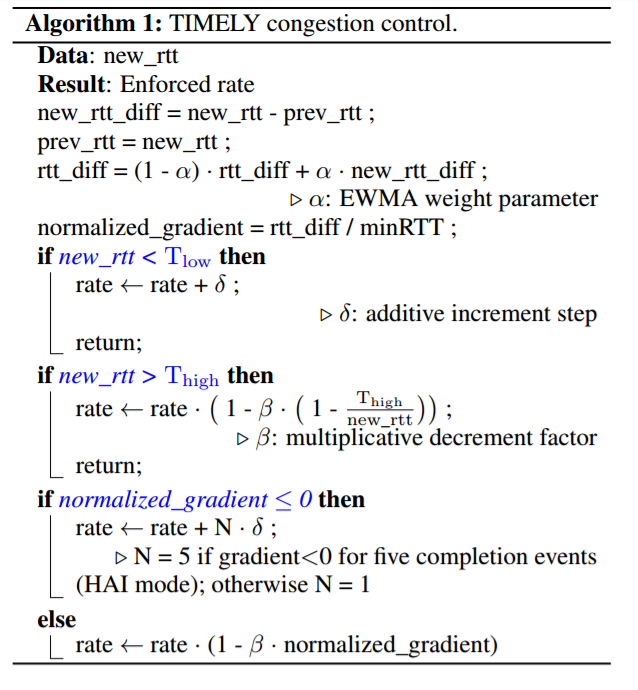
\includegraphics[scale=0.54]{Timely_pseudocode}
  \caption{The Delay Gradient Algorithm described in \textit{Timely: Rtt-based
  Congestion Control for the Datacenter} \cite{mittal2015timely}}
  \label{alg}
\end{algorithm}

\subsubsection{Initial Implementation}


In the very original run right after we implemented the delay gradient scheme
with arbitrarily picked constant, we got a score of $12.51$ (with HAI enabled), which is even worse
than the AIAD scheme. However, we understand the importance of tuning, so we
were quite optimistic with the delay gradient scheme.

\subsubsection{Tuning the Parameters}

We observed that the delay plays an important role in the scoring function and
that the highest scoring teams had the lowest delay, so we
prioritized that when adjusting parameters. Specifically, we decreased our
threshold high parameter.

We initially used Hyperactive increase (HAI) to more aggressively increase the sending
rate after a period of slow growth (where the gradient is negative for $5$
completion events). This enabled us to get higher throughput at the cost of
higher delay. After doing some math on the scoring function, we decided that the
best strategy is to maintain a relatively low delay and then try to maximize the
througput. Thus, we ended up disabling HAI for a less aggressive increase to
achieve a lower delay. 

By looking at the graphs, we saw that there were times when the packet transmission rate dipped to near $0$, so we lower
bounded the packet transmission rate by $1$.

We measured the lowest RTT time observed in the network to be $42$ ms, and
correspondingly set the
\texttt{minRTT} parameter to be $50$ ms. We set the initial rate to be $50$ so
that the algorithm can get a faster head start in transmitting packets. We set
initial \texttt{rtt\_diff} to be $0$ so that it can be updated more quickly to
reflect the gradient of the first few packets.

The rest of the parameters left for us to set are $\alpha$ which controls the
EWMA weight, $\beta$ which is the mutiplicative decrease factor, $\delta$ which
is the additive increase size and $T_{low}$ and $T_{high}$ the two delay
thresholds.

After adjusting these parameters several times, we were able to reach a score of
$30.15$ by setting $\alpha=0.25$, $\beta=0.4$, $\delta=0.1$, $T_{low}=80$ and
$T_{high}=150$.

We then removed the "lowerbounding the packet transmission rate by $1$" part, but
our score decreased because we had long periods of time of $0$ packet
transmission, which led to a slightly lower throughput with approximately the
same delay. 

We then ran a script overnight to vary parameters and got the following result:


% include your own bib file like this:
%\bibliographystyle{acl}
%\bibliography{acl2017}
\bibliographystyle{acl_natbib}
\bibliography{writeup}

\appendix

\section{Supplemental Material}
\label{sec:supplemental}
ACL 2017 also encourages the submission of supplementary material
to report preprocessing decisions, model parameters, and other details
necessary for the replication of the experiments reported in the 
paper. Seemingly small preprocessing decisions can sometimes make
a large difference in performance, so it is crucial to record such
decisions to precisely characterize state-of-the-art methods.

Nonetheless, supplementary material should be supplementary (rather
than central) to the paper. {\bf Submissions that misuse the supplementary 
material may be rejected without review.}
Essentially, supplementary material may include explanations or details
of proofs or derivations that do not fit into the paper, lists of
features or feature templates, sample inputs and outputs for a system,
pseudo-code or source code, and data. (Source code and data should
be separate uploads, rather than part of the paper).

The paper should not rely on the supplementary material: while the paper
may refer to and cite the supplementary material and the supplementary material will be available to the
reviewers, they will not be asked to review the
supplementary material.

Appendices ({\em i.e.} supplementary material in the form of proofs, tables,
or pseudo-code) should come after the references, as shown here. Use
\verb|\appendix| before any appendix section to switch the section
numbering over to letters.

\section{Multiple Appendices}
\dots can be gotten by using more than one section. We hope you won't
need that.

\end{document}
